% !TEX root = ../../Main.tex
\section{Reinforcement Learning}
\label{Section:ReinforcementLearning}

Reinforcement Learning (RL) is the branch of machine learning that studies an agent that interacts with an environment and learns which decisions to make. Unlike supervised learning, it is not given the correct answer for any situation. The agent acts, observes what happens and changes its behaviour according to the reward it receives. Learning therefore happens by trial and error, without labelled examples. This suits problems where the right action is not known in advance but its outcome can be measured. Robotics and finance are two fields where this is the case.

\subsection{Fundamentals and History}

Reinforcement Learning grew out of the combination of several other fields, such as psychology, computer science and control theory. It was inspired by the way humans and animals learn from their environment. In RL, an agent makes decisions and receives rewards or penalties for its actions, with the aim of maximising good outcomes over time. This process is based on operant conditioning, a type of learning studied by psychologists such as B. F. Skinner \cite{skinner_operant_1963}, in which behaviour is shaped by its consequences. Markov Decision Processes (MDPs) were formalised in the late 1950s. They model decision making where the outcomes are partly random and partly under the control of the decision maker. MDPs became the mathematical basis of RL, because they allowed the development of algorithms that learn optimal strategies in complex environments. One of the major advances in RL was Q-Learning, introduced in the late 1980s. It is an algorithm that learns the value of actions in different states, so an agent can make informed decisions without a model of the environment. Q-Learning and Temporal Difference Learning made it possible to apply RL to a wide range of problems, from playing video games better than humans to optimising financial trading strategies \cite{sutton_reinforcement_2018}.

\subsection{Key Concepts and Agent-Environment Interaction}

Reinforcement Learning is about how an agent interacts with its environment. The interaction involves states, actions and rewards. The state \( S_t \) describes the situation of the agent at that moment. When the agent observes \( S_t \), it chooses an action \( A_t \). This action makes the environment transition to a new state \( S_{t+1} \), and the environment gives feedback in the form of a reward \( R_{t+1} \). \Cref{Figure:AgentEnvironment} shows this repeating cycle \cite{sutton_reinforcement_2018}.

\begin{figure}[htb!]
\centering
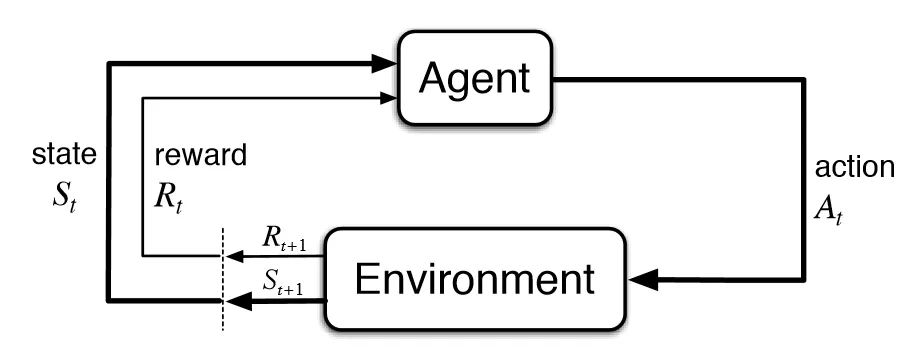
\includegraphics[width=0.6\textwidth]{Images/AgentEnvironment.png}
\caption{Interaction between the agent and the environment in Reinforcement Learning \cite{sutton_reinforcement_2018}.}
\label{Figure:AgentEnvironment}
\end{figure}

The goal of the agent is to maximise the return. The return is the discounted sum of the rewards the agent collects from time \( t \) onwards \cite{sutton_reinforcement_2018}:

\begin{equation}
R_{t+1} + \gamma R_{t+2} + \gamma^2 R_{t+3} + \ldots = \sum_{k=0}^{\infty} \gamma^k R_{t+k+1}
\end{equation}

Here, \( \gamma \) is the discount factor. It sets how much future rewards count compared with immediate ones. A policy \( \pi \) decides the actions of the agent. It can be deterministic, giving one specific action for each state, or stochastic, giving a probability distribution over actions. A main difficulty in RL is the balance between exploration and exploitation. Exploration means trying new actions to find out their effects. Exploitation means choosing actions that are known to give a high reward. A common approach is the \(\varepsilon\)-greedy policy, which usually picks the best-known action but sometimes picks a random one \cite{sutton_reinforcement_2018}. This method needs a discrete set of actions, because it works by picking one of the alternatives at random. When the action is continuous, as in this work, exploration comes instead from adding noise to the action the policy returns. \Cref{Section:DeepReinforcementLearning} describes this approach together with the algorithm that uses it.

Reinforcement Learning is built on the Markov Decision Process (MDP), defined by the tuple \( (S, A, P, R, \gamma) \). Here, \( S \) is the set of all possible states of the environment and \( A \) is the set of actions the agent can take. \( P \) is the transition probability, the probability of moving from state \( s_t \) to state \( s_{t+1} \) after taking action \( a \). \( R \) is the reward function, which gives the reward for that transition, and \( \gamma \) is the discount factor. MDPs rely on the Markov property. It requires the next state to depend only on the current state and action, and not on any earlier ones \cite{sutton_reinforcement_2018}:

\begin{equation}
\label{Equation:MarkovProperty}
P(s_{t+1} | s_t, a_t, s_{t-1}, a_{t-1}, \ldots, s_0, a_0) = P(s_{t+1} | s_t, a_t)
\end{equation}

The reward function matters because it is where the goal of the task is defined. It tells the agent what to achieve, but not how to achieve it. The agent will adopt any behaviour that raises the reward. In trading, the reward is normally computed from profit and loss. This drives the agent towards profitable positions without telling it which positions those are \cite{sutton_reinforcement_2018}.

\subsection{Value Functions and Q-Functions}

The value function of a policy \( \pi \), written \( V^\pi(s) \), is the expected return when starting in state \( s \) and following policy \( \pi \) after that. It is defined as follows \cite{sutton_reinforcement_2018}:

\begin{equation}
V^\pi(s) = \mathbb{E} \left[ \sum_{k=0}^{\infty} \gamma^k R_{t+k+1} \mid S_t = s, \pi \right]
\end{equation}

Here, \( \gamma \) is the discount factor, which sets how much future rewards count compared with immediate rewards. \( \mathbb{E} \) is the expected value, the average of all possible outcomes weighted by their probabilities. The Q-function of a policy \( \pi \), written \( Q^\pi(s, a) \), is the expected return for taking action \( a \) in state \( s \) and following policy \( \pi \) after that. It is defined as follows \cite{sutton_reinforcement_2018}:

\begin{equation}
Q^\pi(s, a) = \mathbb{E} \left[ \sum_{k=0}^{\infty} \gamma^k R_{t+k+1} \mid S_t = s, A_t = a, \pi \right]
\end{equation}

The Bellman equations are named after Richard Bellman, who first formulated them. They give a recursive decomposition of the total cumulative reward an agent can expect, starting from a given state or state-action pair. These equations are the basis of dynamic programming methods in RL. They express the value of a state, or of a state-action pair, in terms of the values of the states that follow it. This recursion is what allows the estimated values to be improved step by step, and it is the basis of convergence for most RL algorithms. The equations are as follows \cite{sutton_reinforcement_2018}:

\begin{equation}
V^\pi(s) = \sum_{a \in A} \pi(a|s) \sum_{s' \in S} P(s'|s,a) \left[ R(s,a,s') + \gamma V^\pi(s') \right]
\end{equation}

\begin{equation}
Q^\pi(s, a) = \sum_{s' \in S} P(s'|s,a) \left[ R(s,a,s') + \gamma \sum_{a' \in A} \pi(a'|s') Q^\pi(s', a') \right]
\end{equation}

\begin{equation}
\label{Equation:RelationshipValueQFunction}
V^\pi(s) = \sum_{a \in A} \pi(a|s) Q^\pi(s, a)
\end{equation}

\Cref{Equation:RelationshipValueQFunction} shows that the value of a state under policy \(\pi\) is the expected value of the Q-function over all possible actions, weighted by the probability the policy gives to each action. For optimal policies, the optimal value function \( V^*(s) \) and the optimal Q-function \( Q^*(s, a) \) give the highest return that can be achieved from any state or state-action pair, respectively. From the Bellman equation, it follows that \cite{sutton_reinforcement_2018}:

\begin{equation}
V^*(s) = \max_{a \in A} \sum_{s' \in S} P(s'|s,a) \left[ R(s,a,s') + \gamma V^*(s') \right]
\end{equation}

\begin{equation}
Q^*(s, a) = \sum_{s' \in S} P(s'|s,a) \left[ R(s,a,s') + \gamma \max_{a' \in A} Q^*(s', a') \right]
\end{equation}

\begin{equation}
V^*(s) = \max_{a \in A} Q^*(s, a)
\end{equation}

By applying these equations again and again, RL algorithms gradually approximate the value function and the Q-function. This guides the agent towards the optimal policy, which is the policy that maximises the expected cumulative reward \cite{sutton_reinforcement_2018}.

\subsection{Methodological Variants and Learning Methods}

Reinforcement learning methods can be divided into groups by the properties of the learning method: model-based or model-free, on-policy or off-policy, and value-based or policy-based. In model-based RL, the algorithm builds a model of the environment to simulate and predict the outcomes of actions. The agent can then plan by predicting the next states. This is possible when the environment is simple enough to be modelled. In model-free RL, the algorithm learns a policy or a value function directly from its interactions with the environment, without building a model of it. Model-free methods are often chosen when the environment is hard to model or when no accurate model is available. Within model-free RL, there are on-policy methods, which learn about the policy that is currently used to make decisions, and off-policy methods, which explore with a different policy while they try to learn an optimal one \cite{sutton_reinforcement_2018}.

Another important distinction is between value-based methods, also called critic-only, and policy-based methods, also called actor-only. Value-based methods, such as Temporal Difference Learning (TD), Q-Learning and SARSA Learning, estimate the value of states or of state-action pairs. The policy is not learned directly. It follows from these values. Temporal Difference learning is the update rule that the other two are built on, and it works in both settings. SARSA is on-policy, because it evaluates the policy it is following. Q-Learning is off-policy, because it evaluates the greedy policy, the one that always takes the highest-valued action, whatever policy it actually follows. To take the highest-valued action, the method has to compare every action, so these methods are limited to discrete sets of actions. Policy-based methods, such as REINFORCE, optimise the policy directly. For this reason they extend to continuous actions, where the policy returns the action itself instead of a value for each possible action. Actor-Critic learning combines the two. It has a policy function (the actor) and a value function (the critic). The policy is improved directly, and the critic gives the value estimates that make those updates stable \cite{sutton_reinforcement_2018}. \Cref{Codes:ActorCritic} gives a detailed implementation.

% !TEX root = ../Main.tex
\begin{algorithm}[htb!]
\DontPrintSemicolon
\KwRequire{$\pi(a \mid s; \theta)$: a differentiable policy, $Q(s, a; w)$: a differentiable $Q$-function, $N$: number of iterations and learning rates $\beta^\theta > 0$ and $\beta^w > 0$}
Initialise policy parameter $\theta^{(0)}$ and $Q$-function parameter $w^{(0)}$\;
Initialise state $s$\;
\For{$n = 0, 1, \ldots, N - 1$}{
    Sample $a \sim \pi(\cdot \mid s; \theta^{(n)})$\;
    Take action $a$, observe state $s'$ and reward $r$\;
    Sample $a' \sim \pi(\cdot \mid s'; \theta^{(n)})$\;
    Compute the TD error: $\delta \gets r + \gamma Q(s', a'; w^{(n)}) - Q(s, a; w^{(n)})$\;
    Update $w$: $w^{(n+1)} \gets w^{(n)} + \beta^w \delta \nabla_w Q(s, a; w^{(n)})$\;
    Update $\theta$: $\theta^{(n+1)} \gets \theta^{(n)} + \beta^\theta \delta \nabla_\theta \ln \pi(a \mid s; \theta^{(n)})$\;
    $s \gets s'$\;
}
\caption{Actor-Critic \cite{sutton_reinforcement_2018}.}
\label{Codes:ActorCritic}
\end{algorithm}

For finite Markov Decision Processes, standard results guarantee that an optimal policy exists and that it can be taken to be deterministic and stationary. These guarantees do not extend to complex, non-stationary environments such as financial markets \cite{sutton_reinforcement_2018}. A raw price series does not have the Markov property. The information a trader uses is spread across the recent history, and is not all contained in the latest quote. RL applied to these markets therefore works with an approximation. Technical indicators and other engineered features put enough of that history into the state for the Markov property to hold approximately. Actor-Critic methods matter here because they are the point where reinforcement learning and neural networks meet. This is the subject of the next section.